\subsection{The CLARA Framework} \label{ssec:framework_clara}
CLARA is a SOA platform designed to build streaming scientific-data analytics applications that allows users to process data as streams across data centers and clouds~\cite{gyurjyan2011clara}.
The framework is used both in JLab for CLAS12 and in NASA for the NASA Information and Data System (NAIADS) and Surface Radiation Budget (SRB) projects~\cite{lukashin2015earth}.

As defined in the Introduction, a data event is the collision of a beam of particles into a target which results in a shower of particles.
A data processing engine or simply engine is a software component that processes the data event, usually reconstructing the data obtained in a specific detector component or providing a secondary functionality.

The CLARA framework consists of four core components: A Data Processing Station, a Pipe, a Data Processing Environment and an Orchestrator:
    \begin{itemize}
        \item \textbf{Data Processing Station}: Usually referred to as a CLARA station, the Data Processing Station acts as a container for a user-made data processing engine.
        In the context of the CLAS12 software, this acts as the container for each engine associated to a hardware component of the CLAS12 detector, with a simple relationship of one station for one engine.
        This station-engine coupling is denoted as a Data Processing Service or simply service, and can be seen in Figure \ref{fig:clara_service}.
        
            \begin{figure}[ht]
                \centering
                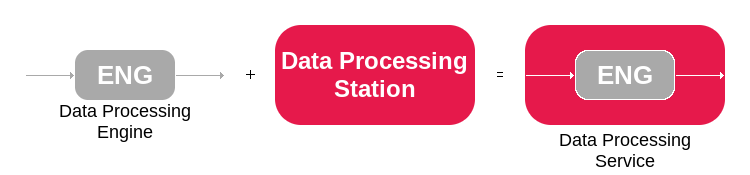
\includegraphics[scale=0.50]{clara/service}
                \caption{\label{fig:clara_service} Data engine and CLARA station coupling.}
            \end{figure}
        
        \item \textbf{Data Stream Pipe}: A data bus based on the xMsg messaging system, which in turn is based on the ZeroMQ protocol~\cite{hintjens2013zeromq}.
        xMsg is a messaging protocol based on the publisher-subscriber pattern which allows for various agents to communicate based on topic subscriptions.
        In the context of the CLAS12 software, the data buses act as pipes between services, allowing one service to send Data Events to another.
        The interaction between stations and pipes can be seen in Figure \ref{fig:clara_station_pipe}.
        
            \begin{figure}[ht]
                \centering
                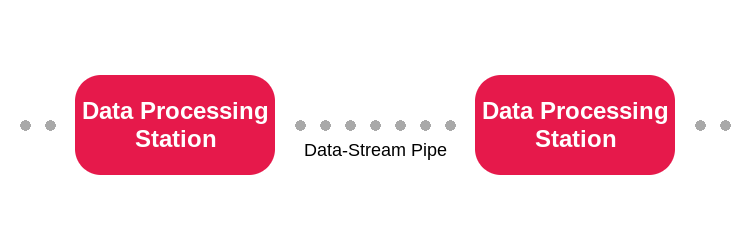
\includegraphics[scale=0.50]{clara/stations_and_pipes}
                \caption{\label{fig:clara_station_pipe} CLARA stations coupled with pipes.}
            \end{figure}
    
        \item \textbf{Data Processing Environment (DPE)}: A DPE is a container unit for one or more services and their corresponding data pipes which acts as a communications hub between the services and the hardware.
        Communication between DPEs can be done using the same data stream pipes.
        Different DPEs can be placed in different computing environments, thus allowing the communication of different services between different machines.
    
        \item \textbf{Data Flow Orchestrator}: The Orchestrator is a system to coordinate the communication between the Data Processing Services via the Data-stream Pipes.
        In CLAS12, the Orchestrator simply forms a straight line between services which is called ``Production Chain'', and each service alters the Data Event as it sees fit to then have the engines following read and write it.
        To setup a production chain such as the one seen in Figure \ref{fig:clara_production_chain}, the Orchestrator must be used to configure each service and pipe to allow the free flow of data.
        
            \begin{figure}[ht]
                \centering
                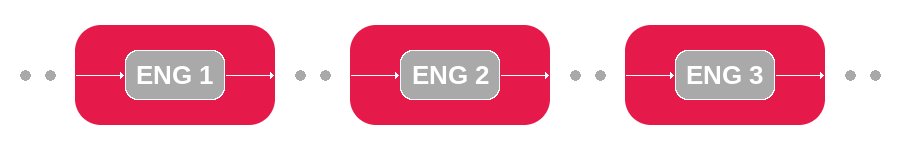
\includegraphics[scale=0.50]{clara/production_chain}
                \caption{\label{fig:clara_production_chain} CLARA production chain.}
            \end{figure}
            
    \end{itemize}